\section{Numerics}\label{sec:numerics}
For many of the works described previously, it is necessary to apply numerical techniques to obtain results. As the Gross--Pitaevskii
equation, given in Eq. \eqref{eqn:gpe}, is used in the majority of the literature cited, we will consider it as the basis for the following discussion. Given the Gross--Pitaevskii equation, as defined by Eqn. \ref{eqn:gpe}, we can see that it is a second order non-linear partial differential equation. Very few exact solutions exist, and the problem must often be tackled by a numerical approach. Though there are many ways to solve such a system numerically, (such as Crank-Nicholson, Trotter-Suzuki), the method I have chosen is the pseudospectral Fourier split-operator \cite{Num:Bauke_cpc_2011}.

If we consider a unitary evolution operator of the form
\begin{equation}\label{eqn:1}
\Psi(\bar{x},t+\tau) = \exp\left[ -\frac{iH\tau}{\hbar}\right]\Psi(\bar{x},t),
\end{equation}
where $H$ is the Hamiltonian, composed of momentum, potential, non-linear, and rotation terms defined in Eq. \eqref{eqn:gpe}, we can solve for the wavefunction over a specified timescale. However, due to error propagation resulting from numerical integration techniques, it is necessary to employ methods that allow for the highest precision while providing results in useful timescales. To allow for this, careful choice of the numerical integration methods must be taken.  If we take the Hamiltonian, $H$, in terms of its components as a combination of position and momentum space functions we obtain
\begin{equation}\label{eqn:2}
\hat{H} = \hat{H}_{\textbf{r}} + \hat{H}_{\textbf{p}} + \hat{H}_{\textbf{L}},
\end{equation}
where we first neglect the angular momentum operator, $\hat{H}_{\textbf{L}}$, and consider only the two other non-commuting parts $\hat{H}_{\textbf{r}}$, containing the position operator, and $\hat{H}_{\textbf{p}}$, containing the momentum operator. This way we can reduce the error in the numerical integration scheme by using 2nd order Strang-splitting as
\begin{equation}\label{eqn:3}
\exp\left[ -\frac{ i\left(\hat{H}_{\textbf{r}} + \hat{H}_{\textbf{p}}\right)\tau}{\hbar} \right] \approx \exp\left[- \frac{i\hat{H}_{\textbf{r}}\tau}{2\hbar} \right]\exp\left[-\frac{i\hat{H}_{\textbf{p}}\tau}{\hbar}\right]\exp\left[ -\frac{i\hat{H}_{\textbf{r}}\tau}{2\hbar}\right].
\end{equation}
The respective functions can be mapped to the Gross--Pitaevskii equation's position, and momentum terms as
\begin{equation}
\hat{H}_{\textbf{r}} = V(\bar{x}) + g\vert\Psi(\bar{x},t)\vert^2\; \hspace{5em} \hat{H}_{\textbf{p}} = \frac{-\hbar^2}{2m}\nabla^2.
\end{equation}
%\hat{H}_{\textbf{L}} = \Omega L,
Following Bauke \textit{et al}. \cite{Num:Bauke_cpc_2011}, we can numerically solve this differential equation as
\begin{equation}
\Psi\left(\textbf{r},t+\tau\right) = \left[\hat{U}_{\mathbf{r}}\left(t+\frac{\tau}{2}\right) \mathscr{F}^{-1} \left[ \hat{U}_{\mathbf{k}}(t+\tau) \mathscr{F} \left[ \hat{U}_{\mathbf{r}}\left(t+\frac{\tau}{2}\right) \Psi\left(\mathbf{r},t\right) \right] \right] \right]  \\ + O\left(\tau^3\right),
\end{equation}
where $\hat{U}_{r}=e^{-i\hat{H}_{r}(t)\tau/\hbar}$ is the time evolution operator in real space, $\hat{U}_{p}=e^{-i\hat{H}_{p}(t)\tau/\hbar}$ in momentum space,  $\mathscr{F}$ and $\mathscr{F}^{-1}$ are the forward and backwards Fourier transform respectively. Following \cite{BK:Pitaevskii_Stringari_2003} and taking the Madelung transform of the wavefunction given by Eq. \eqref{eqn:madelung}, the phase of the condensate may be given by
\begin{equation}
\theta = \theta_c + \theta_i,
\end{equation}
where $\theta_c$ is the unperturbed condensate phase, and $\theta_i$ is the phase pattern to be imprinted. Thus, upon solving for the initial condensate phase, an additional phase pattern can be imprinted at any time by multiplying the wavefunction by the intended phase pattern. This is in line with the phase imprinting method, as previously introduced by Dobrek \textit{et al}. \cite{Vtx:Dobrek_pra_1999}. The underlying theory of the Fourier split-operator method for the Gross--Pitaevskii equation is given by Javanainen \textit{et al}. \cite{BEC:Javanainen_jphysa_2006}, showing how the choice of non-linearity and operator splitting affects the outcome of the method. The authors arrive at the conclusion that treating the non-linearity and potential terms together with the most current wavefunction definition yields results with an error magnitude that matches those obtained in the Schr\"{o}dinger Fourier split-operator case, indicating its applicability to this type of problem.

\begin{figure}
    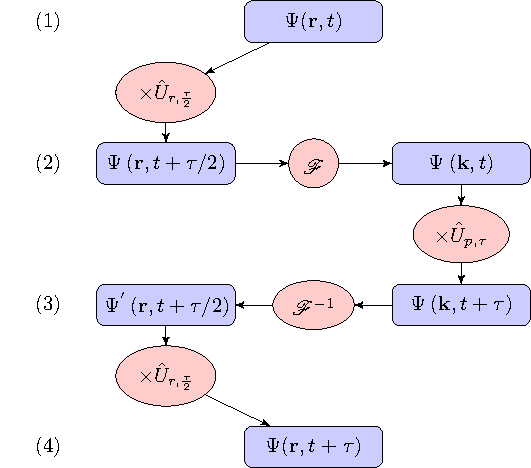
\includegraphics[]{./ch2_numerics/splitop}
    \caption{A single pass through the Fourier split-operator method.}
    \label{fig:num_splitop}
\end{figure}

\section{Angular momentum operators using FSO method}
The Fourier split-operator method described earlier works well in handing cases where the operators live in position or momentum space respectively. However, the angular momentum operators are essentially a combination of both spaces as we deal with each basis respectively. Take, for example, the angular momentum operator along the $z$-axis, given by $L_z = xp_y - yp_x$. To apply $L_z$ we must take not that the $x$ and $y$ components of the wavefunction must be in alternating bases for the evolution. Thus, to apply this operator we must Fourier transform along a single dimension, multiply by the respective operator, take the inverse, and perform this operation along the other dimension.

 This, however, accrues an error not encountered using non-pseudospectral methods. The error can be determined by checking the commutativity of the respective components of the angular momentum operator as
 \begin{align}
 	L_1 = [x p_y,-y p_x] &= [x p_y,-y] p_x  -  y[x p_y,p_x], \\
 				   &= -[-y,x p_y] p_x + y [p_x, x p_y], \\
 				   &= -\left( {\cancelto{0}{[-y,x]}} p_y + x [-y,p_y] \right) p_x + y \left( [p_x,x] p_y + x {\cancelto{0}{[p_x,p_y]}} \right), \\
 				   &= -x {\cancelto{i\hbar}{[-y, p_y]}} p_x + y {\cancelto{-i\hbar}{[p_x,x]}} p_y, \\
 				   &= -i\hbar \left(x p_x + y p_y \right).
 \end{align}

 The complex error term can be seen as, in the case of the implemented evolution, allowing the angular momentum opeartor to change from imaginary time to real-time, and vice-versa in each respective case. To overcome this, we simply swap the application order of the operator components, between even and odd steps during the evolution. Starting with the alternate order we obtain a value of $L_2 = [-y p_x, x p_y] = i\hbar \left(x p_x + y p_y \right)$. Since we are applying this phase to the condensate we can overcome the error of one term by the application of the other, as
 \begin{equation}
 \exp{i L_1}\exp{i L_2} = 1.
 \end{equation}

 Although alternating will provide a cancellation of this error, it can be assumed that for large timesteps the error will have a non-insignificant contribution to the overall dynamics. Thus, for this method to remain accurate we can perform the previous decomposition for a third-order accurate scheme, or use as is for a second-order accurate scheme.

 \subsection{Time evolution}
 To create the initial state for the desired evolution the ground-state of the Hamiltonian needs to be determined as a first step. This can be achieved by evolving the system in imaginary time, where $t\rightarrow it$. This causes all higher energy terms in an initial guess for the condensate wavefunction to decay to zero, leaving the lowest energy state, which corresponds to the ground-state. As effective as this approach may be, the convergence to the lowest lying energy state becomes less effective as the computation approaches the expected value \cite{Vtx:Danaila_pra_2005}. Although many such methods exist, the one that is best suited for this task is that of a Fourier split-operator method. Due to the way the algorithm operates, it is essential to have a large and finely sampled grid in order to resolve both position and momentum of the wavefunction. A minimum grid-size on the order of $2^8$ in 2D for both $X$ and $Y$ dimensions is required. An implementation of such a method at the defined resolution is a straight-forward process using MATLAB, and has been performed for the purpose of this study. However, due to the large computational overhead required to deal with such a calculation, the procedure takes a long time to evolve the system to the necessary degree of accuracy. Therefore, it is necessary to further develop the methods used, and to improve the implementation of this algorithm to leverage the recent advances in computational acceleration.








We can write the wavefunction of a quantum system as a linear superposition of states as
\begin{equation}
     |\Psi \rangle = \displaystyle\sum\limits_{n} C_n |\Psi_n \rangle,
\end{equation}
where $| \Psi_n \rangle$ are a set of basis states for the system, with complex coefficients $C_n$. We next assume a unitary evolution operator of the form
\begin{equation}
    \mathscr{U}(t,t_0) = \exp\left(\frac{-i\mathcal{H}(t-t_0)}{\hbar}\right),
\end{equation}
where $\mathcal{H}$ is the Hamiltonian of the system. To time evolve our system from some time $t_0$ to a final time $t$ we apply the evolution operator to the wavefunction, giving
\begin{equation}
    \mathscr{U}(t,t_0)|\Psi \rangle = \displaystyle\sum\limits_{n} C_n \exp\left(\frac{-i{E_n}(t-t_0)}{\hbar}\right)|\Psi_n \rangle,
\end{equation}
where I have replaced the Hamiltonian operator with the energy eigenvalue of the $n$-th state. It follows from here that each state evolves at a different rate, proportional to its given eigenenergy. Higher energy states will oscillate faster than those of lower energy states. However, to make accurate predictions it is often necessary to deal with a single quantum state, such as the lowest lying state. We can learn much from a quantum system's lowest energy state, and so to evaluate this would be very useful. Taking the evolution operator, we apply a Wick rotation, rotating the time component through $\pi/2$ into the imaginary plane, as $t \rightarrow -it$. Applying this new evolution operator to the wavefunction gives
\begin{equation}
        \mathscr{U^{'}}(t,t_0)|\Psi \rangle = \displaystyle\sum\limits_{n} C_n \exp\left(\frac{-{E_n}(t-t_0)}{\hbar}\right)|\Psi_n \rangle.
\end{equation}
The we have removed the complex term in the operator, which now takes the form of an exponentially decaying operator. When applied to the wavefunction all higher energy terms will decay at a rate faster than lower energy components. This process also causes a loss of probability density, and so the wavefunction must be renormalised after application. Through repeated application of this operator, and a renormalisation afterwards, the quantum system can converge to the groundstate. To begin, however, we must assume an intial guess for the wavefunction, which has some finite overlap with the lowest lying state.











 \section{Vortex tracking}
 To efficiently follow the vortex dynamics, some robust algorithm is needed to track their positions. We could track regions where the density drops to zero. However, this gives very little information on the topological excitation, and may mistake density dips for the presence of such excitations. Thus, one of the most effective ways is to locate the $\pm 2\pi$ charge in the wavefunction phase, which is a signature of quantum vortices. For this, we can assume that around a $2\times 2$ subgrid, the phase rotates from $-\pi$ to $+\pi$ in the presence of a vortex located on the subgrid. After an initial pass to determine the vortex locations closest the nearest grid element, a least-squares fit is performed to more accurately determine the vortex core position. With this, we can accurately the determine the motion of the vortices with high precision.

 To track the vortices during the evolution, the creation of an initial list of vortices is performed, with each given a unique identifier. Assuming the vortex cores can travel a limited distance (some multiple of the grid resolution) between time steps, we can say at subsequent times which vortex has moved to the newly found positions. This is performed through use of a linked list of vortices, each with an assigned unique identifier, associated location, phase winding and on/off flag. A finite boundary is chosen to examine only vortices at the center, which can cause vortices to appear and disappear on the boundary. Thus, any vortex which appears without association to an initial vortex, or any vortex that leaves the boundary, is switched off and remains so for all analysis.
